\scanpage{60}
\figure{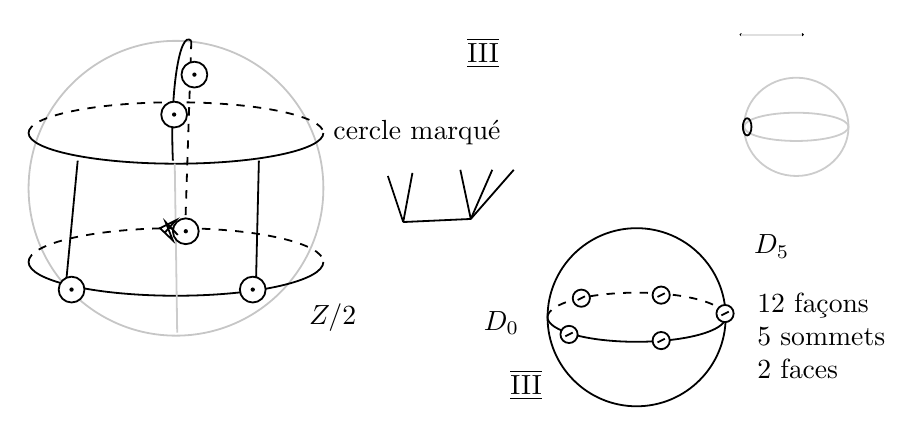
\begin{tikzpicture}[x=.78cm,y=.78cm,line width=.65pt]
\node at (8,6.2){$\underline{\overline{\mathrm{III}}}$};
\draw[gray!45](3,4)circle(2.4);\draw(0.6,4.9)arc(180:360:2.4 and .5);\draw[dashed](.6,4.9)arc(180:0:2.4 and .5);\draw(.6,2.8)arc(180:360:2.4 and .55);\draw[dashed](.6,2.8)arc(180:0:2.4 and .55);
\draw(1.4,4.45)--(1.2,2.35);\draw(4.35,4.45)--(4.3,2.35);\draw(2.95,4.45)..controls(2.9,5.5)and(3.05,6.6)..(3.25,6.4);\draw[dashed](3.25,6.4)--(3.15,3.35);\draw[gray!40](2.98,4.4)--(3.02,1.65);
\foreach \x/\y in {2.97/5.2,3.3/5.85,1.3/2.35,4.25/2.35,3.16/3.3}{\draw[fill=white](\x,\y)circle(.21);\fill(\x,\y)circle(.035);}
\draw(2.82,3.28)--(3,3.48)--(2.74,3.35)--(2.95,3.15)--(2.83,3.45)--(3.03,3.24);
\node[anchor=west]at(5.4,4.9){cercle marqué};\node at(5.55,1.9){$\mathbb Z/2$};
\draw(6.7,3.45)--(7.8,3.5);\draw(6.7,3.45)--(6.45,4.2);\draw(6.7,3.45)--(6.85,4.25);\draw(7.8,3.5)--(7.63,4.3);\draw(7.8,3.5)--(8.15,4.3);\draw(7.8,3.5)--(8.5,4.3);
\fill(12.2,6.5)circle(.025);\fill(13.2,6.5)circle(.025);\draw[gray!25](12.2,6.5)--(13.2,6.5);
\draw[gray!40](13.1,5)ellipse(.85 and .8);\draw[gray!40](13.1,5)ellipse(.85 and .23);\draw(12.3,5)ellipse(.07 and .14);
\draw(10.5,1.9)circle(1.45);\draw(9.05,1.9)arc(180:360:1.45 and .4);\draw[dashed](9.05,1.9)arc(180:0:1.45 and .4);
\foreach \x/\y in {9.6/2.21,9.4/1.62,10.9/2.26,10.9/1.52,11.94/1.96}{\draw[fill=white](\x,\y)circle(.14);\draw(\x-.06,\y-.03)--(\x+.06,\y+.03);}
\node at(8.3,1.8){$D_0$};\node at(12.7,3.05){$D_5$};\node at(8.7,.8){$\underline{\overline{\mathrm{III}}}$};
\node[align=left,anchor=west]at(12.3,1.6){\deleted{12 façons}\\5 sommets\\2 faces};
\end{tikzpicture}}

$9=3+3+1+2$ sommets\\6 faces\\1 cercle marqué

$60=10\times3\times2$ poss. pour $K$

\deleted{\unsure{K}} $(\underset{10}{\text{triangle}}+\underset{3}{\text{sommet marqué}}+\underset{2}{\text{1 sens de rot\unsure{.}}}$

\margin{\uline{12 possibilités} \unsure{qui définissent une} orientation de $K$}
\figure{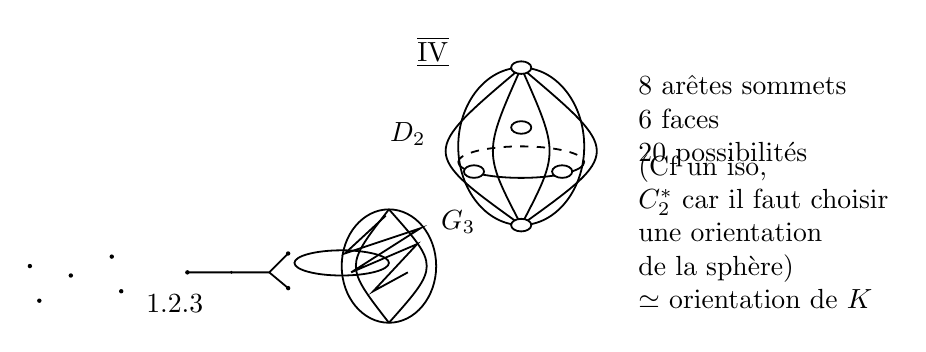
\begin{tikzpicture}[x=.8cm,y=.8cm,line width=.65pt]
\node at(6.4,3.1){$\underline{\overline{\mathrm{IV}}}$};\node at(6,1.8){$D_2$};
\draw(7.8,1.6)ellipse(1 and 1.25);\draw(7.8,2.85)..controls(6.2,1.5)..(7.8,.35);\draw(7.8,2.85)..controls(9.4,1.5)..(7.8,.35);\draw(7.8,2.85)..controls(7.2,1.5)..(7.8,.35);\draw(7.8,2.85)..controls(8.4,1.5)..(7.8,.35);\draw(6.8,1.35)arc(180:360:1 and .25);\draw[dashed](6.8,1.35)arc(180:0:1 and .25);
\foreach \x/\y in {7.8/2.85,7.8/1.9,7.05/1.2,8.45/1.2,7.8/.35}{\draw[fill=white](\x,\y)ellipse(.16 and .1);}
\node[align=left,anchor=west]at(9.5,2){$\unsure{8}$ \deleted{\unsure{arêtes}} sommets\\6 faces\\\uuline{20 possibilités}};
\node[align=left,anchor=west]at(9.5,.25){(\unsure{Cf un iso},\\\deleted{$\unsure{\mathbb C_2^*}$} car il faut choisir\\une orientation\\de la sphère)\\$\simeq$ orientation de $K$};
\draw(5.7,-.3)ellipse(.75 and .9);\draw(4.95,-.25)ellipse(.75 and .2);\draw(5.7,.6)..controls(5,-.3)..(5.7,-1.2);\draw(5.7,.6)..controls(6.5,-.3)..(5.7,-1.2);
\draw(5.65,.5)--(5,-.1)--(6.2,.3)--(5.1,-.4)--(6.15,.05)--(5.45,-.7)--(6,-.4);\node at(6.8,.4){$\unsure{G_3}$};
\foreach \x/\y in {0/-.3,.65/-.45,1.3/-.15,.15/-.85,1.45/-.7}{\fill(\x,\y)circle(.035);}
\draw(2.5,-.4)--(3.8,-.4)--(4.1,-.1);\draw(3.8,-.4)--(4.1,-.65);\fill(2.5,-.4)circle(.035);\fill(3.2,-.4)circle(.025);\fill(4.1,-.1)circle(.035);\fill(4.1,-.65)circle(.035);
\node at(2.3,-.9){\deleted{\unsure{$1.2.3$}}};
\end{tikzpicture}}

choisissons une orientation sur $K$, \deleted{\unsure{donc}} et bornons nous d'abord aux I, II avec pentagones compatibles avec l'orientation. Alors
\diagram{\begin{tikzcd}[ampersand replacement=\&]\deleted{\mathrm{II}}\arrow[r]\&\deleted{\mathrm I}\quad\deleted{\text{deux façons}}\end{tikzcd}}

donnée I $=$ sommet de l'icosaèdre \inserted{gauche $I_{C_\omega}$} $+$ arête \deleted{\unsure{qui en}} \inserted{incidente}, i.e. $\in D_{01}(I_{C_\omega})$
\margin{drapeaux de type 01}

donnée II $=$ sommet de l'icos. g. $+$ face \deleted{\unsure{qui en}} \inserted{incidente}, i.e. $\in D_{02}(I_{C_\omega})$

donnée III $=$ \deleted{\unsure{face}} \inserted{\unsure{tr. de}} \deleted{\unsure{arête}} de l'icos. g., \deleted{$+$ sommet dessus,}

\figure{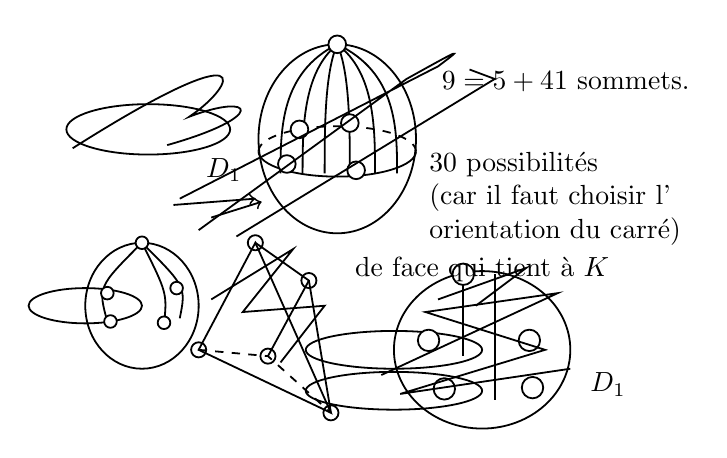
\begin{tikzpicture}[x=.8cm,y=.8cm,line width=.65pt]
\draw(5.7,3.4)ellipse(1.3 and .4);\draw(4.5,3.1)..controls(7.5,5)and(7.1,4.1)..(6.35,3.6)..controls(7.4,4)and(7.6,3.6)..(6,3.15);
\draw(8.7,3.25)ellipse(1.25 and 1.5);\draw(7.45,3.05)arc(180:360:1.25 and .4);\draw[dashed](7.45,3.05)arc(180:0:1.25 and .4);
\foreach \x in {7.8,8.15,8.5,8.9,9.3,9.65}{\draw(8.7,4.75)..controls(\x,4.3)and(\x,3.4)..(\x,2.7);}
\foreach \x/\y in {8.7/4.75,8.1/3.4,8.9/3.5,7.9/2.85,9/2.75}{\draw[fill=white](\x,\y)circle(.14);}
\draw(6.2,2.3)--(10.3,4.4)..controls(10.7,4.7)..(9.8,4.2)--(6.5,1.8);\draw(7.1,1.7)--(11.2,4.2)--(10.8,4.35);\draw[->](6.1,2.2)--(7.4,2.3);\draw[->](6.7,2)--(7.5,2.25);
\node at(6.9,2.75){$D_1$};\node[align=left,anchor=west]at(10.2,4.15){$9=5+4$\deleted{\unsure{1}} sommets.};
\node[align=left,anchor=west]at(10,2.3){30 possibilités\\(car il faut choisir l'\\orientation du carré)};
\draw(5.6,.6)ellipse(.9 and 1);\draw(4.7,.6)ellipse(.9 and .28);\draw(5.6,1.6)..controls(4.9,.9)..(5.05,.35);\draw(5.6,1.6)..controls(6.3,.9)..(6.2,.4);\draw(5.6,1.6)..controls(6,.8)..(5.95,.3);
\foreach \x/\y in {5.6/1.6,5.05/.8,6.15/.88,5.1/.35,5.95/.33}{\draw[fill=white](\x,\y)circle(.1);}
\draw(6.5,-.1)--(7.4,1.6)--(8.6,-1.1)--cycle;\draw(7.4,1.6)--(8.25,1)--(8.6,-1.1);\draw[dashed](6.5,-.1)--(7.6,-.2)--(8.6,-1.1);\draw(8.25,1)--(7.6,-.2);\foreach\x/\y in{6.5/-.1,7.4/1.6,8.25/1,8.6/-1.1,7.6/-.2}{\draw(\x,\y)circle(.12);}\draw(6.7,.7)--(8,1.5)--(7.2,.5)--(8.5,.6)--(7.8,-.3);
\draw(11,-.1)ellipse(1.4 and 1.25);\draw(9.6,-.1)ellipse(1.4 and .3);\draw(9.6,-.75)ellipse(1.4 and .3);\draw(10.7,1.15)--(10.7,-.2);\draw(11.2,1.1)--(11.2,-.9);\foreach\x/\y in{10.7/1.1,10.15/.05,11.75/.05,10.4/-.72,11.8/-.7}{\draw[fill=white](\x,\y)circle(.17);}\draw(9.4,-.5)--(12.2,.8)--(10.1,.5)--(12,-.1)--(9.7,-.8)--(12.4,-.4);\draw(10.3,.7)--(11.7,1.2)--(10.9,.6);\node at(13,-.65){$D_1$};
\node at(11,1.18){\deleted{\unsure{de face qui tient à $K$}}};
\end{tikzpicture}}
\diagram{\begin{tikzcd}[ampersand replacement=\&, row sep=small]
\deleted{D_0}\arrow[r]\&\deleted{D_1}\quad\deleted{\text{cinq façons}}\\
\deleted{D_1}\arrow[r]\&\deleted{D_2}\\
D_{01}\arrow[r]\&D_0\\
D_{01}\arrow[r,no head]\&D_1\\
D_{02}\arrow[r,no head]\&D_0\\
D_{02}\arrow[r,no head]\&D_2\quad\deleted{\uuline{\unsure{bipartité}}}
\end{tikzcd}}
\mspage{59}
